\chapter{Ausblick}
\section{API / Bindings in seprartem Projekt}
\label{sec:separatebindings}
Beim TiM55x-Service habe ich unbewusst die HFTM-\acrshort{lidar}-Library bis zum Contract durchdrücken lassen. Dies habe ich exemplarisch so beibehalten. Das Problem ist folgendes: der Servant, der mit diesen Service kommuniziert, braucht alle Objekte vom Contract. Die Dependencies eines Services werden beim standardmässigen bauen eines Jars aber nicht eingepackt. Für die Ausführung des Services mit dem Befehl \ctexttt{java -jar paketname.jar} packen wir aber sowieso alle Dependecies in ein Jar, damit lediglich diese Datei aufs Zielsystem deployed / kopiert werden muss. Der Grössenunterschied ist allerdings immens und deshlab sollte ein Servant nicht dieses so genannte Fat-Jar als Depedency reinziehen.

\subsection{Verbesserungsvorschlag}
Das Java-Package \ctexttt{bindings} auslagern in ein eigenes Maven-Projekt. Damit hat man eine klare Separation zwischen Service und \acrshort{api} / \Gls{contract}. 

\section{Fehlerbehandlung innerhalb der Services}
Die entwickelten Services müssen in einem weiteren Schritt noch fehlertoleranter gemacht werden. So muss beispielsweise der TiM55x-Service beim Verlieren der Verbindung zum Sensor, in einem regelmässigen Intervall versuchen, die Verbindung wieder aufzunehmen. Dies ist wichtig weil in dieser Architektur die Fehler nicht mehr zentral ersichtlich sind. Es kann ja auch sein, dass jemand angefordert hat, keine weiteren Daten zu liefern. Weshalb kommen also keine Daten mehr - weil es so sein soll, oder weil ein Fehler vorliegt? Der Service müsste beim Verlieren des Sensor einen Status auf ,,Rot'' schalten, damit ein Monitoring-Service im System beim Ausfallen einer Komponente die richten Entscheidungen trifft, und in unserem Kontext beispielsweise den Roboter anhält oder langsamer fahren lässt.

\section{Servant abkürzen über eine Referenz}
Mit dem Betreuer wurde während der Arbeit mehrfach darüber diskutiert, ob der Datenaustausch von Service zu Service immer über den Servant abgewickelt werden muss, oder ob sich der Weg auch aus Performance-Gründen abkürzen liesse. Den auch beim ,,reinen durchreichen'' einer Nachricht muss die in Bezug auf CPU-Rechenleistung teure De- und Serialisierung trotzdem gemacht werden. Selbstverständlich könnte sich der konsumierende Service ja einfach wie der in diesem Dokument beschriebene Servant verhalten bzgl. Importieren des Service-Contracts, aber genau das wollen wir verhindern. Ein Service darf in dieser Ideologie keine direkte Abhängigkeit von einem anderen Service haben.

Vor der Implementierung des EdgeDetection-Services dachten wir aber daran, dass dies trotzdem ein Use-case sein könnte. Schliesslich hat die Software der HFTM das ja vorher in einem Rutsch gemacht.
Schlussendlich hatte der Betreuer die Idee mithilfe des Servants einem Service über dessen Intent mitzuteilen, wo er seine Daten abholen kann und wie das Mapping seiner Struktur mit der Derjenigen des übergebenen Topics zusammenpasst. Der Service müsste anschliessend eine Subscription auf das übergebene Topic machen und die Daten entsprechend mappen. 
Der Betreuer hat die Idee in einem E-Mail niedergeschrieben. Sie ist im Anhang \ref{sec:servant-abkuerzern-referenz} zu finden. 

Die Idee, diesen Ansatz für die Services TiM55x und EdgeDetection zu verwenden, mussten aber aufgegeben werden. Die Struktur vom TiM55x passt überhaupt nicht mit der Struktur von der EdgeDetection zusammen. Denn der TiM55x liefert Polarkoordinaten und die EdgeDetection benötigt und liefert Daten im Kartesischen Koordinatensystem.

\section{Performance Serialisieren / Deserialisieren}
Im Sprint 3 habe ich versucht, mit dem Tool VisualVM herauszufinden, wo die meiste Leistung verbraucht wird. Wie vermutet taucht beim Anzeigen der Hotspots überall die Serialisierungs-Library \ctexttt{snakeyaml} auf:
\begin{figure}[H]
	\centering
	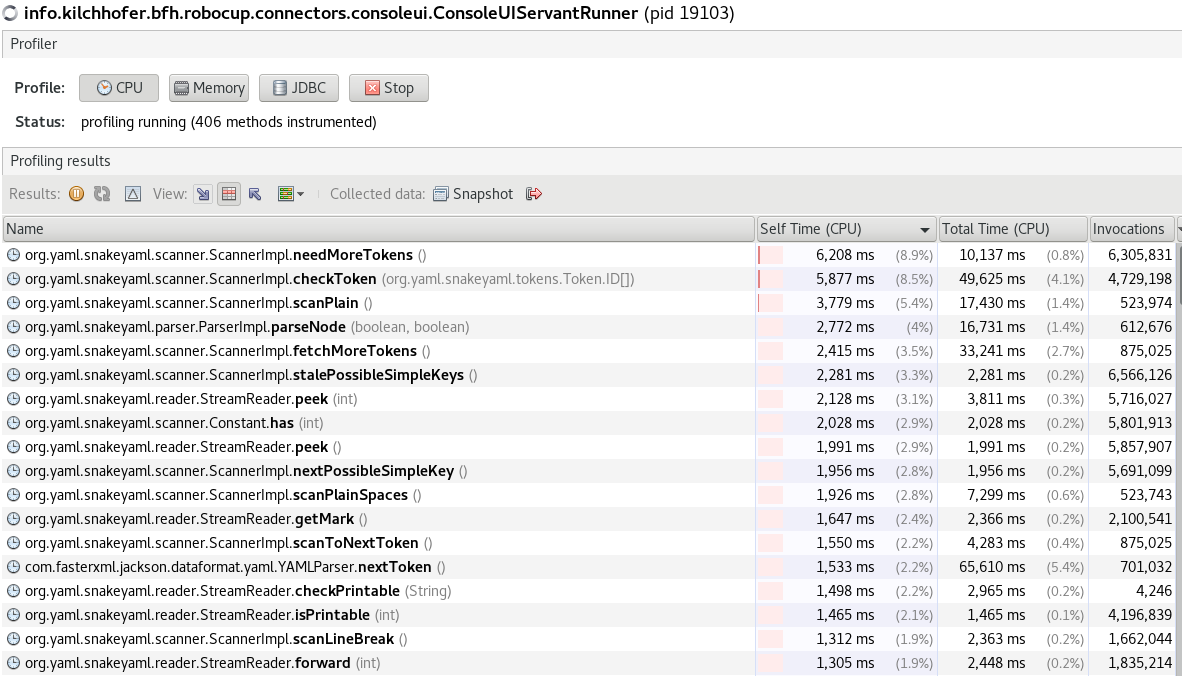
\includegraphics[width=1.0\textwidth]{img/profiling.png}
	\caption{Versuch mit VisualVM den Servant zu Profilen}
	\label{fig:profiling-servant}
\end{figure}
Um die Daten aus dem Screenshot \ref{fig:profiling-servant} zu bewerten bräuchte ich vermutlich mehr Java-Erfahrung. Aber sollten man durch die Entwicklung der vielen Services an die Grenzen stossen in Bezug auf CPU-Performance, wäre vermutlich angebracht im GatewayClient auf eine andere Art die Daten zu Serialisieren. Ich würde mir in diesem Moment dann als erstes mal die Protocol buffers von Google anschauen.